\exercise

Assume you are given a set of 6 strings \{{\tt aa}, {\tt ad}, {\tt bc}, {\tt
bd}, {\tt ca}, {\tt dc}\} and you wish to construct a minimal ordered perfect
hash function, where the order is the alphabetic one.  Assume that
$rank(x)=3,4,5,6$ for the characters $x=a,b,c,d$ respectively. Given a string
$x'x''$ of two characters, we let the two random functions required by the
design of MOPHF as $$h_1(x'x'') = 3 \cdot rank(x') \cdot rank(x'') \bmod 13$$
and $$h_2(x'x'') = rank(x') + rank(x'') \bmod 13,$$ (so $m = 13$). Design a
proper $g(t)$ to construct the final $h(t)$, if this is possible, given $h_1$
and $h_2$ above.

\solution

Hash values for $x'x''$ are shown in \autoref{tab:opmphf-hashes}. The values of
$h$ are the the rank of each string. To find the values of $g$ such that
$$h(x'x'') = g(h_1(x'x'')) + g(h_2(x'x''))$$ we first need to build the
undirected graph $G$ where each node corresponds to a value in the codomain of
$h_1$ (and $h_2$) and the edges to the pairs $(h_1(x'x''), h_2(x'x''))$, one for
each string $x'x''$ in the dictionary. This graph $G$ (represented in
\autoref{fig:opmphf-graph}) is acyclic, so we can construct the function $g$
using the algorithm {\tt LabelAcyclicGraph}(G), obtaining the function in
\autoref{tab:opmphf-g}.

%
\begin{table}[t]
  \begin{subtable}{\textwidth}
    \centering
    \begin{tabular}{c|c|c||c|c|c}
      $x'x''$ & $h_1(x'x'')$ & $h_2(x'x'')$ & $h(x'x'')$ & $g(h_1(x'x''))$ & $g(h_2(x'x''))$ \\ \hline
      {\tt aa} & $3 \cdot 3 \cdot 3 \bmod 13$ & $3 + 3 \bmod 13$ & 0 & 0 & 0 \\
      {\tt ad} & $3 \cdot 3 \cdot 6 \bmod 13$ & $3 + 6 \bmod 13$ & 1 & 3 & 4 \\
      {\tt bc} & $3 \cdot 4 \cdot 5 \bmod 13$ & $4 + 5 \bmod 13$ & 2 & 4 & 4 \\
      {\tt bd} & $3 \cdot 4 \cdot 6 \bmod 13$ & $4 + 6 \bmod 13$ & 3 & 0 & 3 \\
      {\tt ca} & $3 \cdot 5 \cdot 3 \bmod 13$ & $5 + 3 \bmod 13$ & 4 & 0 & 4 \\
      {\tt dc} & $3 \cdot 6 \cdot 5 \bmod 13$ & $6 + 5 \bmod 13$ & 5 & 5 & 0 \\
    \end{tabular}
    \caption{}
    \label{tab:opmphf-hashes}
  \end{subtable}
  \vspace{1em} \\
  \begin{subtable}{\textwidth}
    \centering
    \begin{tabular}{c|ccccccccccccc}
      $t$    & 0 & 1 & 2 & 3 & 4 & 5 & 6 & 7 & 8 & 9 & 10 & 11 & 12 \\\hline
      $g(t)$ & 0 & 0 & 3 & 0 & 0 & 0 & 0 & 0 & 4 & 4 & 3  & 0  & 5  \\
    \end{tabular}
    \caption{}
    \label{tab:opmphf-g}
  \end{subtable}

  \caption{{\bf (a)} Values of $h_1$, $h_2$, $h$, and $g$ computed for each
  string. {\bf (b)} The function $g$.}

\end{table}
%
\begin{figure}[t]
  \centering
  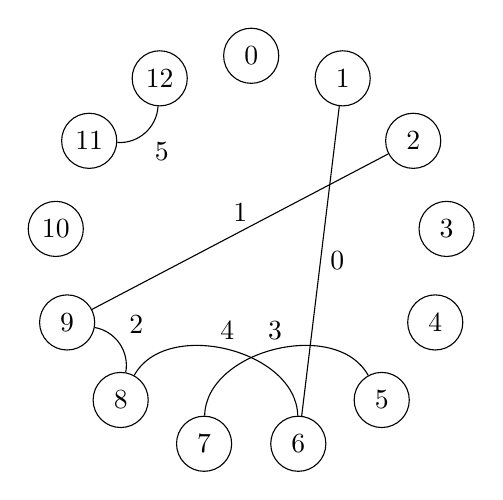
\begin{tikzpicture}
    \def \radius {2.5cm}
    \def \angle {-27.692307692}

    \node[draw, circle, minimum size=0.7cm, inner sep=0] (0) at (0*\angle + 90:\radius) {0};
    \node[draw, circle, minimum size=0.7cm, inner sep=0] (1) at (1*\angle + 90:\radius) {1};
    \node[draw, circle, minimum size=0.7cm, inner sep=0] (2) at (2*\angle + 90:\radius) {2};
    \node[draw, circle, minimum size=0.7cm, inner sep=0] (3) at (3*\angle + 90:\radius) {3};
    \node[draw, circle, minimum size=0.7cm, inner sep=0] (4) at (4*\angle + 90:\radius) {4};
    \node[draw, circle, minimum size=0.7cm, inner sep=0] (5) at (5*\angle + 90:\radius) {5};
    \node[draw, circle, minimum size=0.7cm, inner sep=0] (6) at (6*\angle + 90:\radius) {6};
    \node[draw, circle, minimum size=0.7cm, inner sep=0] (7) at (7*\angle + 90:\radius) {7};
    \node[draw, circle, minimum size=0.7cm, inner sep=0] (8) at (8*\angle + 90:\radius) {8};
    \node[draw, circle, minimum size=0.7cm, inner sep=0] (9) at (9*\angle + 90:\radius) {9};
    \node[draw, circle, minimum size=0.7cm, inner sep=0] (10) at (10*\angle + 90:\radius) {10};
    \node[draw, circle, minimum size=0.7cm, inner sep=0] (11) at (11*\angle + 90:\radius) {11};
    \node[draw, circle, minimum size=0.7cm, inner sep=0] (12) at (12*\angle + 90:\radius) {12};

    \path (1) edge node[right] {0} (6);
    \path (2) edge node[above] {1} (9);
    \path (6) edge[bend right=75] node[above] {4} (8);
    \path (7) edge[bend left=75] node[above] {3} (5);
    \path (8) edge[bend right=45] node[above right] {2} (9);
    \path (11) edge[bend right=45] node[below right] {5} (12);
  \end{tikzpicture}
  \caption{Graph corresponding to the strings {\tt aa}, {\tt ad}, {\tt bc}, {\tt
  bd}, {\tt ca}, {\tt dc}.}
  \label{fig:opmphf-graph}
\end{figure}
